\documentclass[a4paper,11pt]{article}

% Always keep your main language last
\usepackage[norsk,nynorsk,samin,british]{babel}

\usepackage{_sty/UiT}
\usepackage{_sty/IMS}
\usepackage{MAT-2202/MAT-2202}

% ============================================================ 
% COURSE INFORMATION
% ============================================================

% This is old to be removed

% Default time is 09:00 - 13:00 | Uncomment and change the line below  \visif neccecary
% \newcommand{\examtime}{15:00--19:00}
\newcommand{\location}{\aasgard}
\newcommand{\permittedAids}{%
    \supportMaterial{c,r}}
\newcommand{\paper}{squares}
\newcommand{\pages}{} % Sets the total number of pages manually. Uncomment if neccecary
\newcommand{\contact}{\MariusOve}
\newcommand{\mobile}{}
\settoggle{isVisit}{true} % Uncomment this line if examinator / person in charge is visiting
\newcommand{\visitWhen}{ca. kl. 11:00}
\settoggle{showVisit}{false} %Uncomment if unknown when visit

% \newcommand{\ExerciseNumber}{1}

\Published{2016}{06}{01}% YEAR {dddd} MONTH {01 - 12} DAY {01 - 31} 
% \Deadline{2018}{11}{27}% Has to be set, not visible if exam

\settoggle{isLF}{true}
\settoggle{isLF}{false} % Comment this line to show solutions

\settoggle{isEksamen}{false}
\settoggle{isEksamen}{true} % Uncomment this if used for exams

\settoggle{isEksamenUtsatt}{false}
% \settoggle{isEksamenUtsatt}{true} % Uncomment this line if Re sit exam (kont / utsatt eksamen)

% ============================================================ 
% v OWN COMMANDS AND PACKAGES BELOW HERE v
% ============================================================

\frontpageUiTsetup{%
    % All the options in UiTsetup are listed below. They all have four defaults:
    %
    %   1)  Commented out   2) empty  3) auto  4) value 
    %
    %  1) If an option is commented out, the associated line is not shown in the
    %     table
    %  2) If a line is empty then the associated line is shown, but the value 
    %     itself is empty.
    %  3) If the command auto is used then the default value is used. This 
    %     depends on the various commands, for the values that have default 
    %     values they are listed beside the command. See below for more details..
    %  4) If you write in any value, that value is displayed in the table as 
    %     normal.
    %
    % ---------------------------|-------------------------
    %         Input              |     Visual Output    
    % ---------------------------|-------------------------
    %    % CourseCode = {auto},  | 
    %    % CourseCode = {},      | 
    %    % CourseCode = {MAT101},| 
    %      CourseCode = {auto},  |     Exam in: & \courseCode \\
    %      CourseCode = {},      |     Exam in: & \\
    %      CourseCode = {MAT101},|     Exam in: & MAT101 \\
    % ---------------------------|-------------------------
    %
    Language = {english}, %auto = language defined by babel
    Exam = {true}, % Is this an exam? true / false
%    Exercise = {true}, % Is this an exercise? true / false
%    ExerciseNumber = {1} % Which exercise number is this?
    CourseCode = {auto}, % auto = \courseCode (defined in courseCode.sty, e.g. MAT-1001.sty)
    CourseName = {auto}, % auto = \courseName (defined in courseCode.sty, e.g. MAT-1001.sty)
    Year = {2017}, % No auto setting for this, as it might change on recompilation
    Month = {6}, % No auto setting for this, as it might change on recompilation
    Day = {1},% No auto setting for this, as it might change on recompilation
%    DeadlineYear = {2020},
%    DeadlineMonth = {12},
%    DeadlineDay = {22},
    StartHour = {9}, % Input is 1,2,...,24 (auto = 9) (DONT USE 01, 02 etc)
%    StartMinute = {15}, % Default is 0, auto = 0
    EndHour = {auto}, % If no EndHour, EndHour = (StartHour + DurationHours) % 24
%    EndMinute = {0}, % Default is 0, auto = 0
    % Note: you can EITHER use DeadlineYear, DeadlineMonth, DeadlineDay, 
    %                 OR       DurationHours, DurationMinutes, DurationDays
    %                 NOT both
    DurationHours = {4}, % default = 0, auto = 4 
%    DurationMinutes = {3680}, % Set the number of minutes the exam should last
%    DurationDays = {1}, % Set the number of days the exam should last
    Location = {\AA{s}gardveien 9},
    ApprovedAids = {\supportMaterial{c,r}},
    Sheets = {\Squares}, % Use \Squares, \Lines or write nothing
    Pages = {}, % Uses auto = pagecount, write in number to override
    ContactID = {mariusove}, % Use the ID from IMS.sty, you CAN use a full name, but PLEASE UPDATE IMS.sty instead.
% You CAN write in a mobile number, but PLEASE UPDATE THE IMS.sty and use ID INSTEAD
    Mobile = {auto}, % blank, auto or mobile number
    Phone = {auto}, % blank, auto or mobile number
    Visit = {true}, % Use true if the lecturer will visit during exam, otherwise false,
%    Visit = {false}, % Visit MUST be true or false
    VisitWhen = {Approx 11} % Write in the approx time the lecturer will visit
}

\begin{document}

% \FrontpageUiT[norsk]

\frontpageUiT

% \include{MAT-2202-Exam-bok-31-05-2017}

% \include{MAT-2202-Exam-nyn-31-05-2017}

\titlebox[nynorsk]

\Problem{($\SI{20}{\percent}$)}

A \emph{vertex cover} for a graph
$\Gamma = (V, E)$ is a collection 
of vertices that meets every edge. 
%
The graph in \cref{fig:MAT-2202-31-05-2017-problem-1}
%
\begin{figure}[H]\centering
    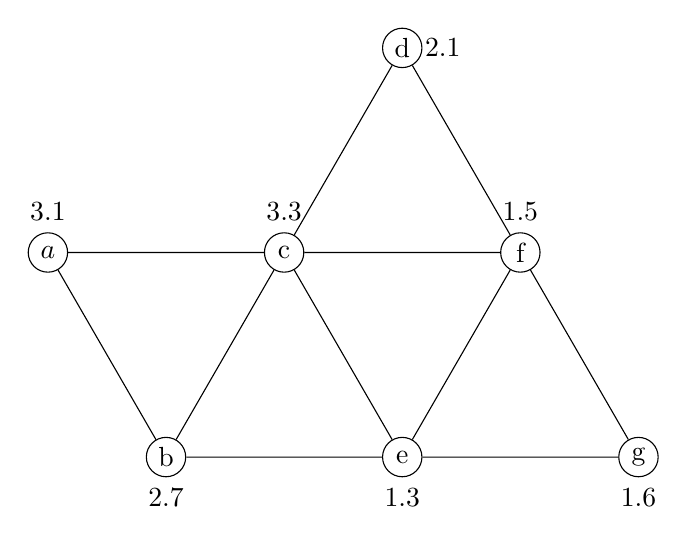
\begin{tikzpicture}[every node/.style={draw,circle,minimum size=5mm,inner sep=0}]
    \def\distance{3cm}
        \node[label=above:{$3.1$}] (a) at (0,0) {$a$};
        \path (a) ++(-60:\distance) 
              node[label=below:{$2.7$}] (b) {b}; 
        \path (a) ++(0:\distance)%
              node[label=above:{$3.3$}] (c) {c}; 
        \path (c) ++(60:\distance)%
              node[label=right:{$2.1$}] (d) {d};
        \path (c) ++(-60:\distance)%
              node[label=below:{$1.3$}] (e) {e};
        \path (c) ++(0:\distance)% 
              node[label=above:{$1.5$}] (f) {f};
        \path (f) ++(-60:\distance)%
              node[label=below:{$1.6$}] (g) {g};
        
    \draw (a) -- (c) -- (d) -- (f) -- (g) -- (e) -- (b) -- (a) (c) -- (b) (c) -- (f) -- (e) -- (c);
    \end{tikzpicture}
    \caption{}
    \label{fig:MAT-2202-31-05-2017-problem-1}
\end{figure}
%
has a weight function $\fun[w]{V}{\R^+}$ on the vertices.
The weights are marked in the sketch. The total weight of vertex cover is the sum of the weights of the vertices in the cover.

\begin{subproblem}
    For the graph in \cref{fig:MAT-2202-31-05-2017-problem-1} exhibit the steps of a greedy algorithm
    to obtain a vertex cover with small total weight.
\end{subproblem}

\begin{subproblem}
    For the graph in \cref{fig:MAT-2202-31-05-2017-problem-1}, formulate the problem of obtaining a vertex cover 
    with minimum total weight as an Integer Linear Programming problem.
\end{subproblem}

\newpageNotLF

\Problem{($\SI{30}{\percent}$)}

\begin{subproblem}
    Establish that the function
    %
    \begin{equation}
        f(x, y) = x^2 - 2xy + 7y^2 + \sin(x),
    \end{equation}
    %
    is strictly convex everywhere.
\end{subproblem}

\begin{subproblem}
    For the function $f$, compute the Newton step $\vp$ at
    $\vx_0 = \mat{0 & 0}\tran$. Is this Newton step a descent 
    direction?
\end{subproblem}

\begin{subproblem}
    Explain briefly how Newton's method applied to a strictly convex
    $C^2$ function may be modified so that it becomes a reliable downhill
    search. The proposed modification should ensure that full Newton
    steps are take when close to a minimum point.
\end{subproblem}


\Problem{($\SI{20}{\percent}$)}

\bgroup \newcommand{\dollar}[1]{$\$\,#1$}

A company plans to build six factories over the next
four years. It will build factories of a fixed size, at a cost that it has forecast
to vary somewhat over the years. The number of new factories justified by
projected demand, and the forecast cost to build a factory, are given in \cref{tab:MAT-2202-31-05-2017-problem-3}.
%
\begin{table}[H]
    \centering
    \caption{}
    \label{tab:MAT-2202-31-05-2017-problem-3}
    \begin{tabular}{c c c}
        \toprule
             Year & New factories at end of year & Cost per factory\\
        \midrule
             $0$ & $\leq 1$ & \dollar{32\text{m}} \\
             $1$ & $\leq 2$ & \dollar{32\text{m}} \\
             $2$ & $\leq 5$ & \dollar{32\text{m}} \\
             $3$ & $=6$ & \dollar{32\text{m}} \\
        \bottomrule
    \end{tabular}
\end{table}
%
A factory can be built within a single year, but no more than two can be built
in a year. During any year in which the company builds one or two factories, 
it incurs a lump-sum cost of \dollar{2\text{m}}. We ignore interest charges 
formulatea dynamic programming model to minimise the total cost of the capacity
expansion, but do not solve it.
\egroup

\newpageNotLF


\Problem{($\SI{30}{\percent}$)}

\begin{subproblem}
    The linear program
    %
    \begin{align*}
        \minus x + y & \to \min \\
           -   x + y & = 1 \\
               x , y & \geq 0,
    \end{align*}
    %
    is in standard form. Sketch the feasible set $S$ in a rectangular coordinate
    system, and mark off the basic solution(s), the basic feasible solution(s), and
    the optimal solution(s) in the sketch.
\end{subproblem}

\begin{subproblem}
    Show that if $\vx_1$ and $\vx_2$ are optimal solutions of an $LP$ problem, then
    $\vx_3 = \num{0.5}\vx_1 + \num{0.5}\vx_2$ is also an optimal solution of the same LP problem.
\end{subproblem}

\begin{subproblem}
    The LP problem
    %
    \begin{alignat*}{2}
                 3 x_1 -            x_2 - x_3 &&\longrightarrow &\min \\
        \phantom{2}x_1 + \phantom{2}x_2 + x_3 &&{} + s_1 \geq & \ 2 \\
                 2 x_1 +          5 x_2 + x_3 &&{} + s_2 \geq & \ 7 \\
                   x_1,             x_2,  x_3,s_1,e_2 && \geq & \ 0, 
    \end{alignat*}
    %
    is in standard form. The basic feasible solution
    %
    \begin{equation}
        \vx 
        = \mat{x_1 & x_2 & x_3 & s_1 & s_2}\tran 
        = \mat{  1 &   1 &   1 &   1 &   0}\tran,
    \end{equation}
    %
    is given. Perform a single step of the simplex method to obtain from 
    $\vx$ a new basic feasible solution that improves the objective.
\end{subproblem}

\end{document}